\fancychapter{State-of-the-Art}
\label{sec:introduction:background}

In this chapter, the main State-of-the-Art concepts regarding the engineering behind an \acs{mppt} charger and solar panels are explained. More specifically, it addresses key challenges such as: what is a solar panel, \acs{mppt} algorithms, \acs{dc}-\acs{dc} converter types, and battery charging techniques. Additionally, it contains a market analysis.  


\section{Solar Panels}

    \ac{pv} panels convert solar irradiance into electrical energy. A \acs{pv} panel consists of multiple solar cells electrically connected in series and/or parallel to achieve the desired voltage and current levels. As in conventional electrical systems, the interconnection topology directly affects the panel's electrical characteristics: series connections increase output voltage, while parallel connections increase output current~\cite{bendib_survey_mppt_methods}.

    \acs{pv} panels connected in series operate at higher voltage levels, reducing conduction losses in interconnecting cables and improving the efficiency of the \acs{dc}-\acs{dc} conversion stage. 
    Moreover, power converters designed for high voltage and low current operation are generally less complex and more cost-effective than those operating at low voltage and high current. 
    However, series configurations are more sensitive to partial shading or panel failure, as the output current of the entire string is limited by the weakest module~\cite{Shading_Effect_PV_Modules_2011}. 
    In contrast, parallel configurations provide improved tolerance to shading and faults but result in higher current levels and increased conduction losses.
    In this project, the series/parallel configuration of the solar panels will not be changed, since \ac{tsb} already defines it, but it is important to understand the implications of each configuration. 

    Each cell is made of a semiconductor material, usually silicon. This semiconductor is doped with phosphorus, a group V element, to create a negative type layer. On the other side, a layer is doped with boron, a group III element, to create a positive type layer. This creates a p-n junction, which is essential for the photovoltaic effect~\cite{photovoltaics_System_Design}.

    \begin{figure} [!ht]
        \centering
        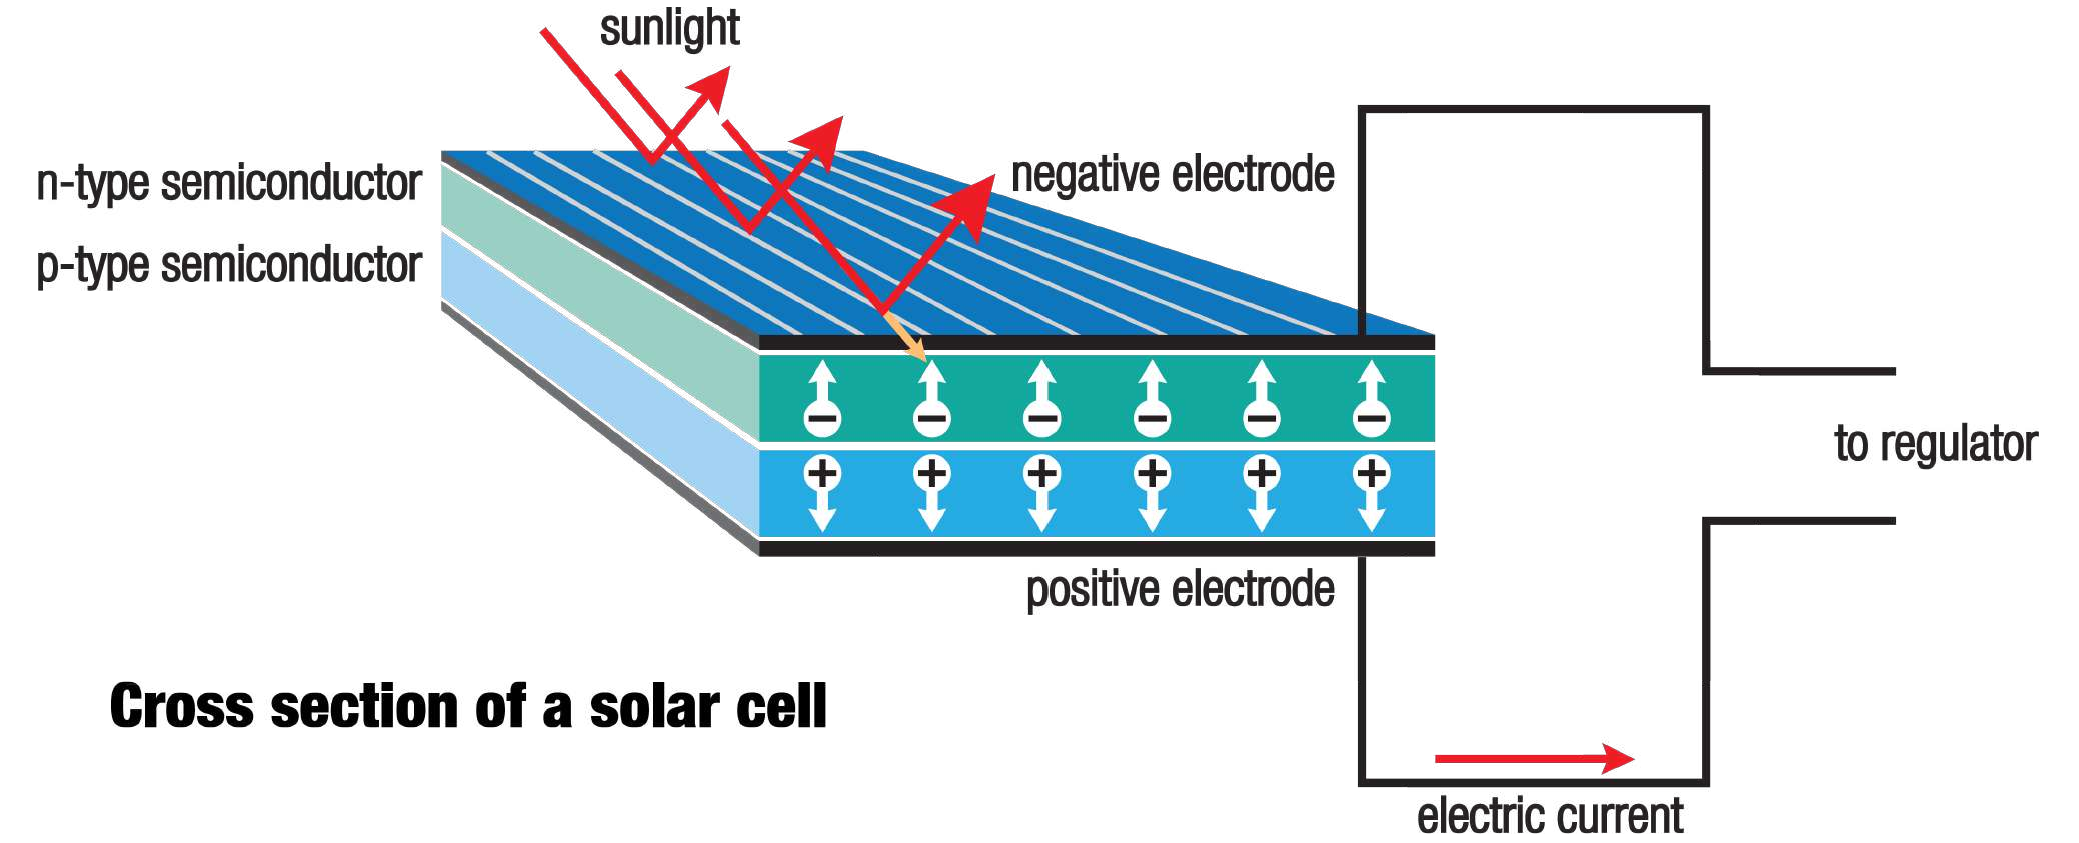
\includegraphics[width=0.60 \textwidth]{Images/Background/solar_cell.pdf}
        \qquad
        \caption{Principle of operation of a solar panel~\cite{imagem_solar_panel}.}
        \label{fig:Solar_Cell}
    \end{figure}

    When sunlight reaches the solar cell, the semiconductor absorbs the photon's energy. This energy excites electrons, allowing them to escape their atomic bonds and create electron hole pairs. The electric field at the p-n junction drives these free electrons toward the n-type layer and holes toward the p-type layer, generating an electric current when the cell is connected to an external circuit~\cite{photovoltaics_System_Design}, Figure~\ref{fig:Solar_Cell}.

    The energy generated results in voltage and current outputs that are not constant. Voltage and current are interdependent, therefore, a variation in one parameter leads to a corresponding variation in the other. This relationship is nonlinear and can be characterized by a current-voltage (I-V) curve. Furthermore, the power output also varies with operating conditions and can be represented by a power-voltage (P-V) curve. Figure~\ref{fig:i-v,p-v} shows both curves.
    In both curves, there is a specific point where the power output is maximized, known as the \ac{mpp}. This point corresponds to a unique combination of voltage and current, denoted as $V_{mpp}$ and $I_{mpp}$, respectively. Operating the solar panel at this point ensures optimal energy extraction under a given condition.

    \begin{figure} [!ht]
        \centering
        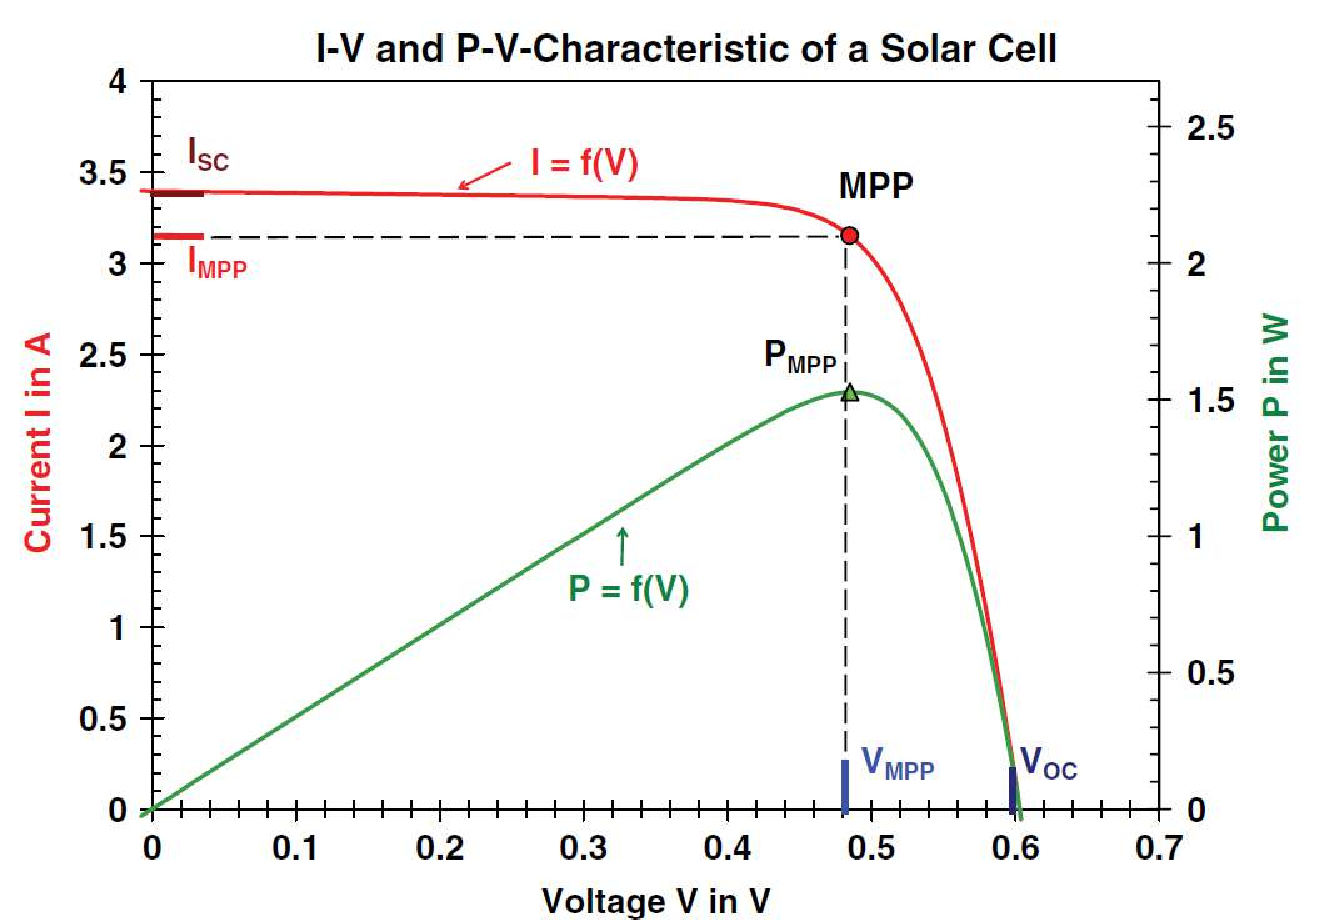
\includegraphics[width=0.50 \textwidth]{Images/Background/i-v,p-v.pdf}
        \qquad
        \caption{I-V and P-V curves of a solar panel~\cite{photovoltaics_System_Design}.}
        \label{fig:i-v,p-v}
    \end{figure}


    The characteristic curves of a solar panel depend on several factors, including material quality, solar cell type, and environmental conditions such as temperature, solar irradiance, wind, and shade. It is noted that under partial shading conditions, it is possible to have multiple local maximums, but overall, there is still only one true \ac{mpp}~\cite{Comparison_PV_Array_MPPT_Techniques_2007}.

    As shown in Figure~\ref{fig:irradiance_i-v}, changes in solar irradiance affect the solar panel's I-V and P-V curves. Higher irradiance produces more power mainly by increasing the panel's current output. In contrast, temperature has the opposite effect (Figure~\ref{fig:temperature_i-v}). Higher temperatures decrease power output, mainly by reducing the panel's voltage output. 

    \begin{figure}[!ht]
        \centering
        \begin{subfigure}[b]{0.48\textwidth}
            \centering
            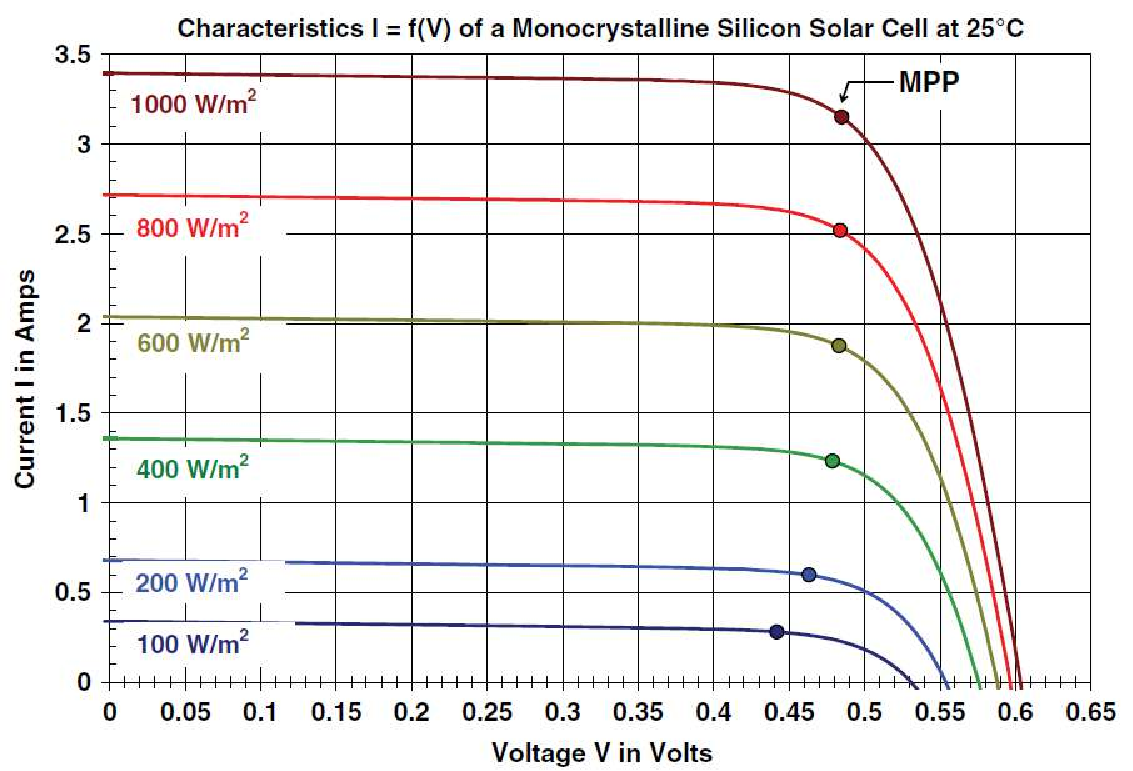
\includegraphics[width=1 \textwidth]{Images/Background/irradiance_i-v.pdf}
            \qquad
            \caption{Cell temperature of 25~ºC and variable Irradiance. }
            \label{fig:irradiance_i-v}
        \end{subfigure}
        \hfill
        \begin{subfigure}[b]{0.48\textwidth}
             \centering
            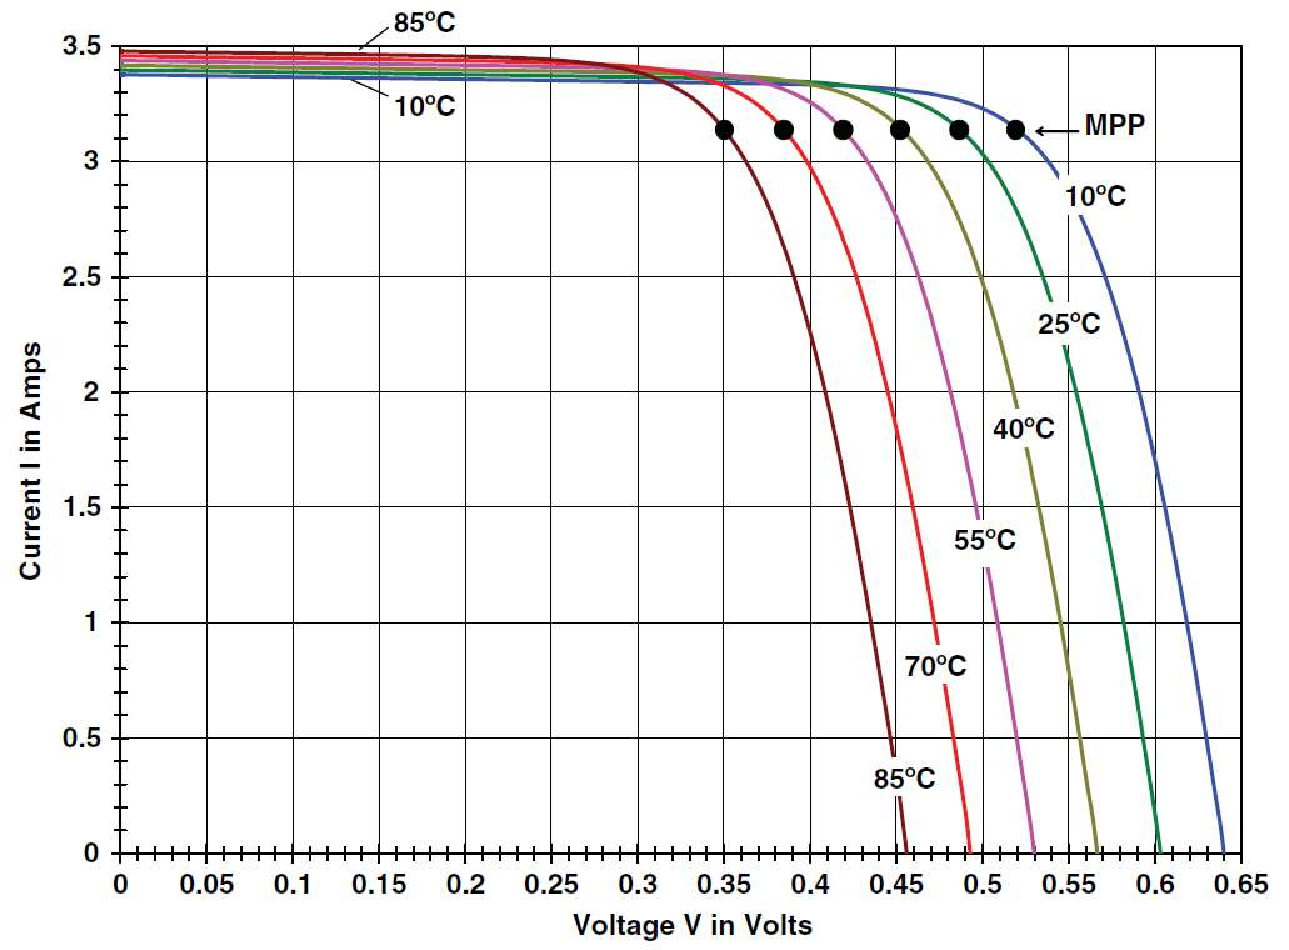
\includegraphics[width=1 \textwidth]{Images/Background/temperature_i-v.pdf}
            \qquad
            \caption{Irradiance of 1~$\mathrm{kW/m}^2$ and variable temperature.}
            \label{fig:temperature_i-v}
        \end{subfigure}
        \caption{I-V curves under different conditions~\cite{photovoltaics_System_Design}.}
        \label{fig:iv-pv-side-by-side}
    \end{figure}
    

    Both environmental conditions have a meaningful impact on the \acs{mpp} of the solar panel and, therefore, on the system's power output. To maximize the power extracted by the solar panels, a classic power converter, such as a buck converter with a fixed duty cycle, is inefficient because neither the current nor the voltage remains constant under varying conditions. Instead, an \acs{mppt} charger is used, which will find the \acs{mpp} and operate the solar panel at that point while sensing the changes caused by the environment.

\section{Maximum Power Point Tracker (MPPT)}

    There are two main types of "trackers": mechanical trackers and electrical trackers. Both aim to maximize the energy extracted from a photovoltaic panel, but in different ways. Mechanical trackers are movable structures that follow the sun's movement, maximizing the panel's exposure to sunlight throughout the day. These devices are complex, expensive, and inefficient, so most research has focused on electrical “tracking” of the \ac{mpp}.

    An electrical \acf{mppt} charger is a device that is used to optimize the power output from solar panels by continuously tracking and adjusting the operation point of the panels to ensure they operate at their \ac{mpp}. 

    To achieve this goal, an \ac{mppt} charger usually consists of a \acs{dc}-\acs{dc} converter, a microcontroller, and sensors (Figure~\ref{fig:block diagram mppt}). The sensors are used to measure the input/output variables of the control system (typically voltage and current). The microcontroller processes the information from these sensors and runs an algorithm to determine whether the \ac{mpp} has been reached or how to act on the system to move toward the \ac{mpp}. In the second case, the microcontroller generates a signal to control the \acs{dc}-\acs{dc} converter, which adjusts its operation accordingly.
 
    \begin{figure} [!ht]
        \centering
        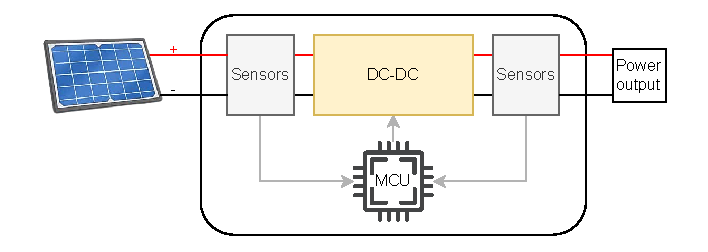
\includegraphics[width=0.65 \textwidth]{Images/Background/Block diagram.drawio.pdf}
        \qquad
        \caption{Simplified structure of an \acs{mppt} charger.}
        \label{fig:block diagram mppt}
    \end{figure}
    
    The output can be connected to different types of loads, like batteries, \acs{dc} loads or inverters. This project focuses on battery charging applications.

\section{MPPT Algorithms}
    There are plenty of \ac{mppt} algorithms, each one with its own advantages and disadvantages. The choice of algorithm depends on the specific application, the desired performance, and the available resources. 
    In this work, the aim is to extract the maximum possible energy from a solar panel installed on a moving boat, which produces I-V curve variations due to rapid changes in irradiance from inclination, orientation, and clouds, as well as temperature changes from waves and wind.
    For these reasons, tracking speed and accuracy are the most important factors to consider.

    With this in mind, we briefly review the most relevant algorithms to identify the most suitable option for this project.

    \subsection{Constant Voltage (CV)}
        The \ac{cv} algorithm is the simplest and most inefficient method. It works by operating the solar panel at a fixed voltage. This reference voltage is used to calculate the duty cycle of the \acs{dc}-\acs{dc} converter to maintain the solar panel's operating point.
        

         Well known variants improve performance by setting the reference voltage to a fraction of the open-circuit voltage (typically 71-78\%)~\cite{Comparison_PV_Array_MPPT_Techniques_2007}. This voltage is obtained by briefly disconnecting the panel from the load, increasing reference accuracy and efficiency. Another variant uses a fraction of the short-circuit current as the reference~\cite{MPPT_Comparison_techniques}.
         

        Although both methods are simple and cost-effective, they are inherently inefficient because they must interrupt energy production during measurement phases. However, alternative implementations address this limitation through proxy measurement techniques employing dummy cells or diodes, whose physical properties closely approximate those of standard solar cells, thereby enabling continuous power generation during measurement acquisition~\cite{Comparison_PV_Array_MPPT_Techniques_2007}~\cite{Optimum_Operating_Point_Tracker_2004}. Still, the \ac{mpp} is not always located at the same percentage of the open circuit voltage or short circuit current, leading to a lack of accuracy and therefore lower efficiency~\cite{Comparative_study_MPPT_algorithms_2000}.


    \subsection{Perturb and Observe (P\&O)}
        The \ac{peo} method is widely used in commercial products and is the basis of many advanced algorithms. Its popularity lies in its simplicity, low cost, and ease of implementation.

        As its name indicates, the algorithm perturbs the voltage of a \acs{pv} array and observes the resulting effect on the output power~\cite{chermitti2012improvement}. If an increase in voltage leads to an increase in output power, the operating point is moving toward the \ac{mpp}, and the algorithm continues to increase the voltage. Conversely, if output power decreases, the operating point moves away from the \ac{mpp}, and the algorithm reverses the perturbation direction~\cite {PeO_and_Newton_Raphson_Comparison,Look-Up-Table_VS_PeO}. Figure~\ref{fig:PeO_flowchart} shows the algorithm flowchart.
                

        The main drawback of this algorithm is that it oscillates around the \ac{mpp}, causing power losses. This oscillation can be reduced by decreasing the perturbation step size, but this also reduces the algorithm's tracking speed. This results in an inherent trade-off between tracking speed and accuracy~\cite{MPPT_Comparison_techniques,Comparison_PV_Array_MPPT_Techniques_2007}.

        Another weal know issue of \ac{peo} is that it can get confused in rapidly changing environmental conditions, like fast irradiance changes caused by clouds. In this case, the algorithm can misinterpret the power change caused by environmental variation as its own perturbation, leading it to move away from the \ac{mpp} instead of toward it~\cite{Comparison_PV_Array_MPPT_Techniques_2007}. For example, if the perturbation is in the wrong direction but irradiance increases, the power output increases, and the algorithm continues perturbing in the wrong direction (Figure~\ref{fig:PeO_Divergence}).

        \begin{figure}[!ht]
            \centering
            \begin{minipage}[b]{0.49\textwidth}
                \centering
                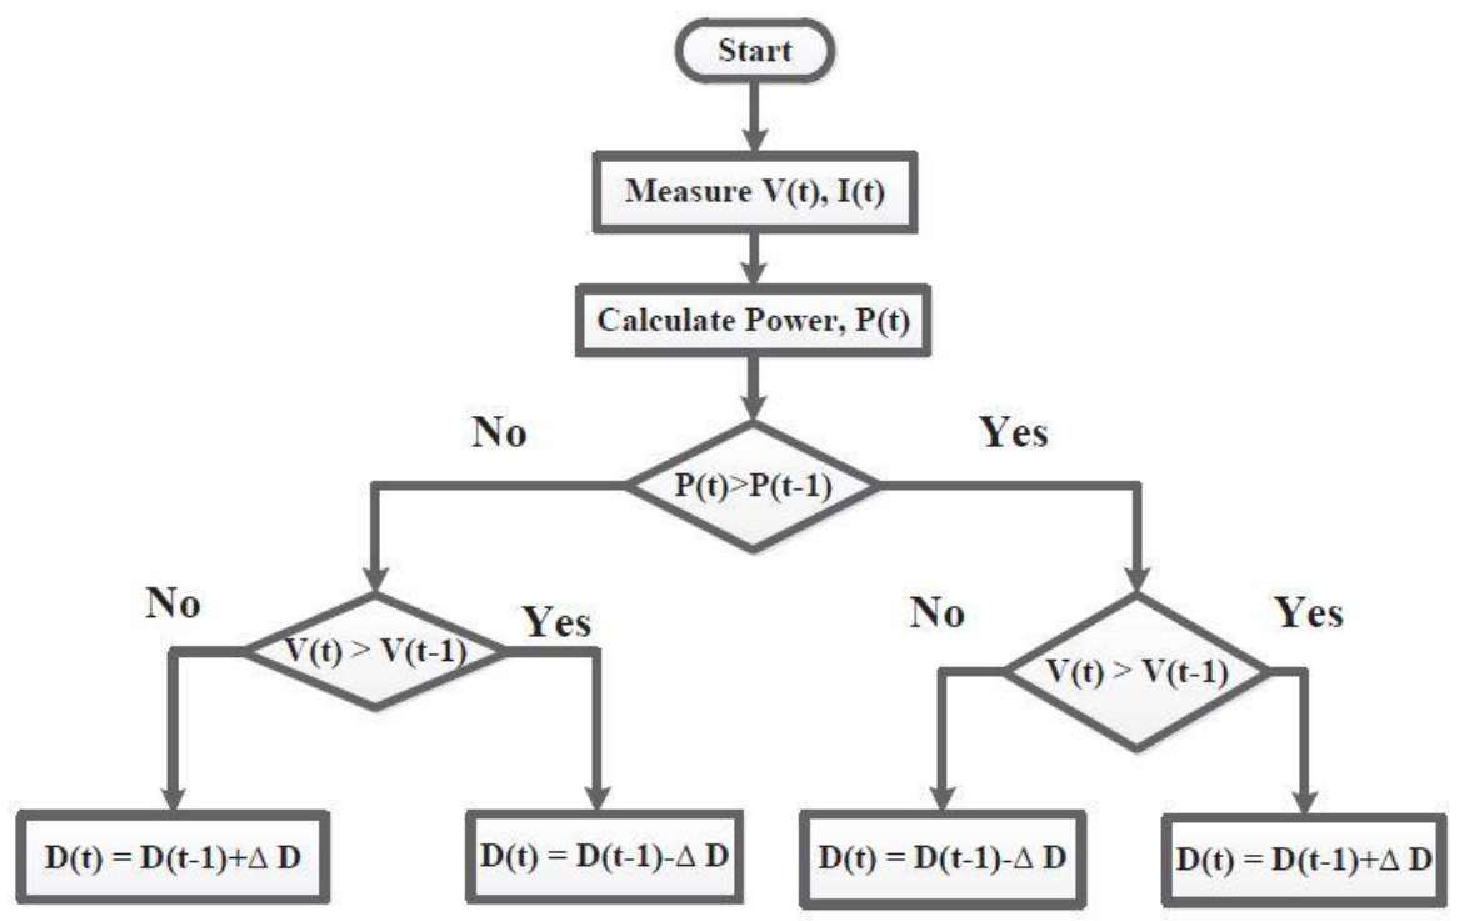
\includegraphics[width=\textwidth]{Images/Background/PeO.pdf}
                \caption{Flow chart of the classic version of Perturb and Observe algorithm~\cite{Look-Up-Table_VS_PeO}.}
                \label{fig:PeO_flowchart}
            \end{minipage}
            \hfill
            \begin{minipage}[b]{0.49\textwidth}
                \centering
                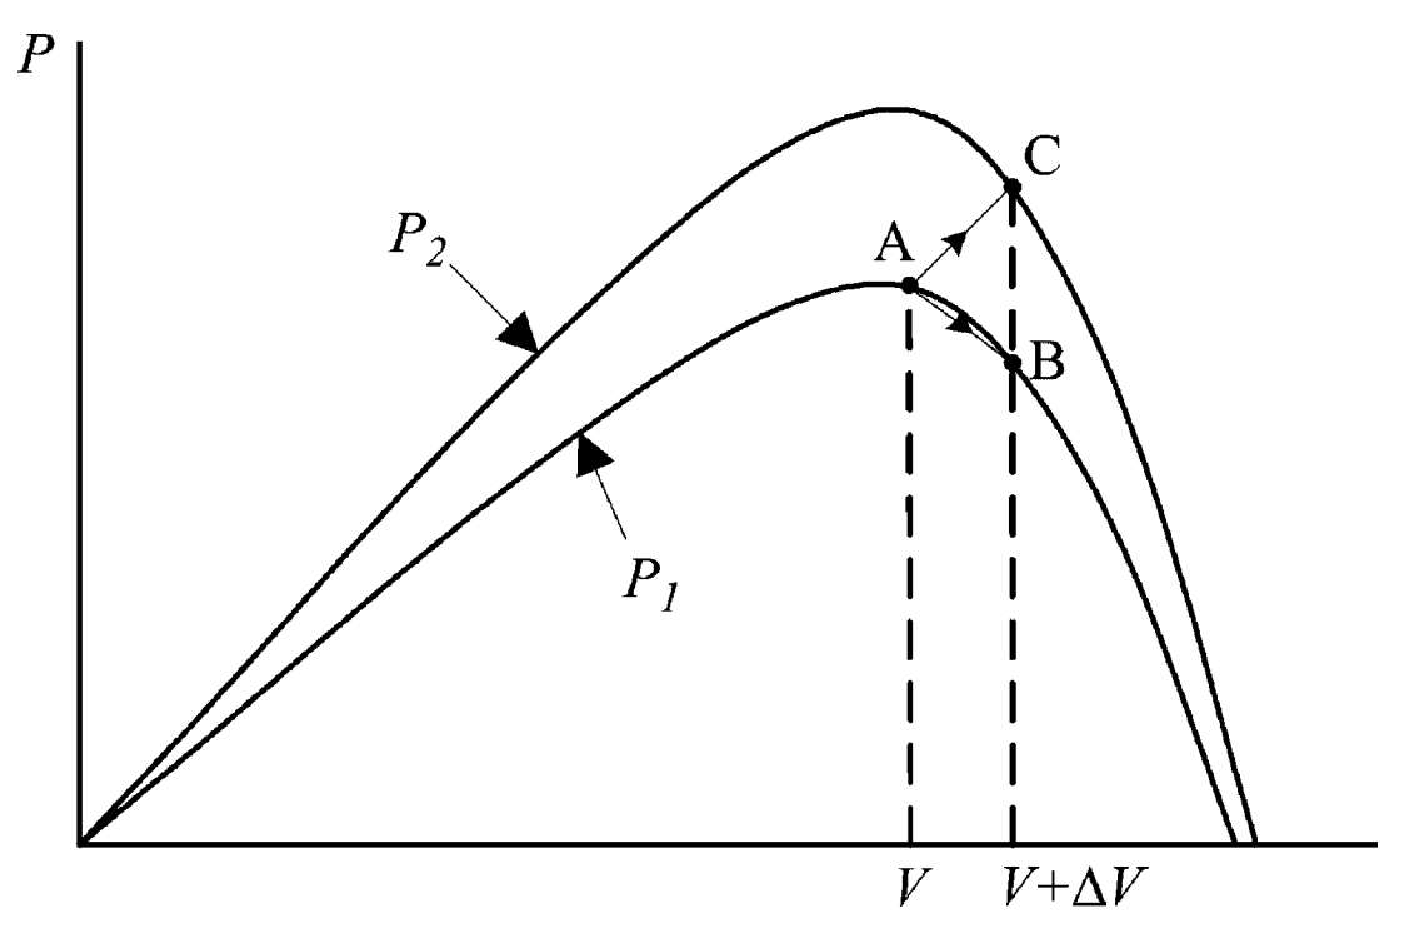
\includegraphics[width=\textwidth]{Images/Background/fast_change.pdf}
                \caption{Divergence of \ac{peo} from MPP as shown in~\cite{4112312}.}
                \label{fig:PeO_Divergence}
            \end{minipage}
        \end{figure}

        To address this limitation, an additional condition can be incorporated into the algorithm that evaluates two consecutive measurements of $\Delta P$ and $\Delta V$. Specifically, when the signs of consecutive $\Delta P$ measurements do not follow the signs of $\Delta V$, this indicates that the observed power variation results from environmental disturbances rather than the algorithm's perturbation. Consequently, the voltage adjustment is suppressed. This refined variant is designated the two-point algorithm or improved \ac{peo} method~\cite{bendib_survey_mppt_methods}.

        There are other variations of \ac{peo} algorithm that improve its performance, like Variable Step Size \ac{peo} (VSS-\ac{peo}), the three-point \ac{peo}, a-factor \ac{peo}, and more. Unfortunately, due to the scope of this work, it is not possible to explain all of them.


    \subsection{Incremental Conductance (IncCond)}
        The \ac{incond} algorithm is another widely used \ac{mppt} method due to its accuracy and ability to track the \ac{mpp} under rapidly changing environmental conditions.
        
        This algorithm is based on the fact that at the \ac{mpp}, the derivative of power with respect to voltage is zero. Given the solar panel output voltage and current, the algorithm can calculate the conductance (I/V) and the incremental conductance (dI/dV)~\cite{Intelligent_PV_Module_2006}. 
        
        The following formulas in Equation~\ref{eq:inc_cond_mpp} show the equation on which this algorithm is based on. 

        \begin{equation}
            \frac{dP}{dV} = \frac{d(V \cdot I)}{dV} = I + V \frac{dI}{dV} \rightarrow \frac{1}{V} \times \frac{dP}{dV} = \frac{I}{V} + \frac{dI}{dV}
            \label{eq:inc_cond_mpp}
        \end{equation}

        At the \ac{mpp} point, the slope of the P-V curve is zero, which means that the negative of the conductance, $-I / V$, is equal to the incremental conductance, $dI / dV$, (Figure~\ref{fig:IncCond_graph}). The algorithm compares these two values to determine if the operating point is at, to the left, or to the right of the \ac{mpp}~\cite{MPPT_Comparison_techniques}\cite{Comparison_PV_Array_MPPT_Techniques_2007}:

        \begin{equation}
            \begin{aligned}
            \frac{dP}{dV}=0 \quad&\Longleftrightarrow\quad \frac{dI}{dV}=-\frac{I}{V}
            \qquad &&\text{at MPP} \\[4pt]
            \frac{dP}{dV}>0 \quad&\Longleftrightarrow\quad \frac{dI}{dV}>-\frac{I}{V}
            \qquad &&\text{left of MPP} \\[4pt]
            \frac{dP}{dV}<0 \quad&\Longleftrightarrow\quad \frac{dI}{dV}<-\frac{I}{V}
            \qquad &&\text{right of MPP}
            \end{aligned}
            \label{eq:inc_cond}
        \end{equation}


        Based on these conditions, the algorithm adjusts its operating point (increasing or decreasing the voltage) using a variable step size based on the instantaneous conductance relative to the incremental conductance, Figure~\ref{fig:IncCond_flowchart}. For example, as suggested in~\cite{Comparison_PV_Array_MPPT_Techniques_2007}, the step size can be calculated using a proportional integral (PI) controller with zero as input reference and error defined as:

        \begin{equation}
            e = \frac{I}{V} + \frac{dI}{dV}
        \end{equation}

        Comparative analysis shows that the \ac{incond} algorithm performs better than the \acs{peo} method. This outcome is expected, as the Incremental Conductance technique was developed specifically to address the limitations inherent in the \acs{peo} approach~\cite{Intelligent_PV_Module_2006}. For example, the \ac{incond} method eliminates the oscillation problem around the MPP that is characteristic of the \acs{peo} method. Additionally, \ac{incond} performs better under rapidly changing environmental conditions, such as sudden irradiance variations, because it uses derivative information that is less sensitive to transient disturbances~\cite{bendib_survey_mppt_methods}. The downside is increased complexity and, therefore, more parameters, which increases simulation and tuning time. Also, it uses fractions, which can be very demanding for \acp{mcu}.

        \begin{figure}[!ht]
            \centering
            \begin{minipage}[b]{0.41\textwidth}
                \centering
                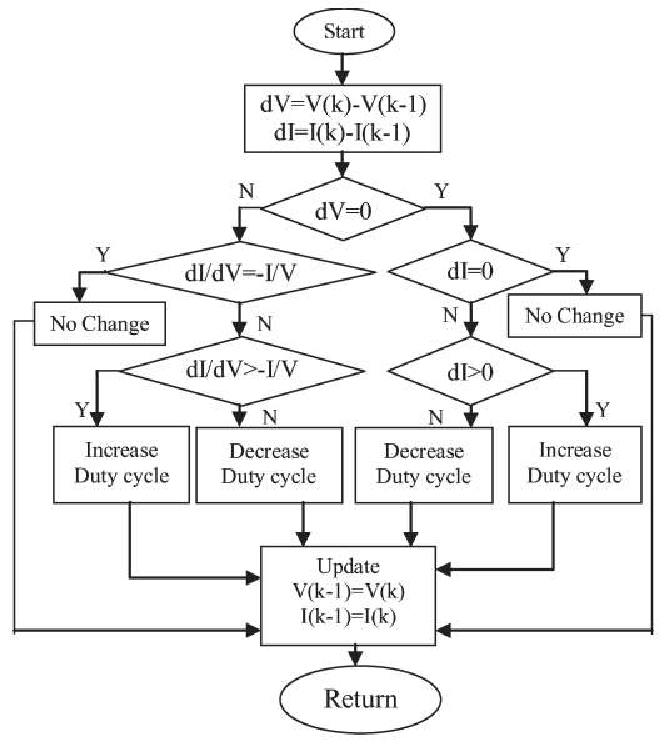
\includegraphics[width=\textwidth]{Images/Background/IncCond_flow.pdf}
                \caption{Flowchart of the \ac{incond} method with direct control (for a buck converter)~\cite{IncCond_MPPT_Cuk_2011}.}
                \label{fig:IncCond_flowchart}
            \end{minipage}
            \hfill
            \begin{minipage}[b]{0.41\textwidth}
                \centering
                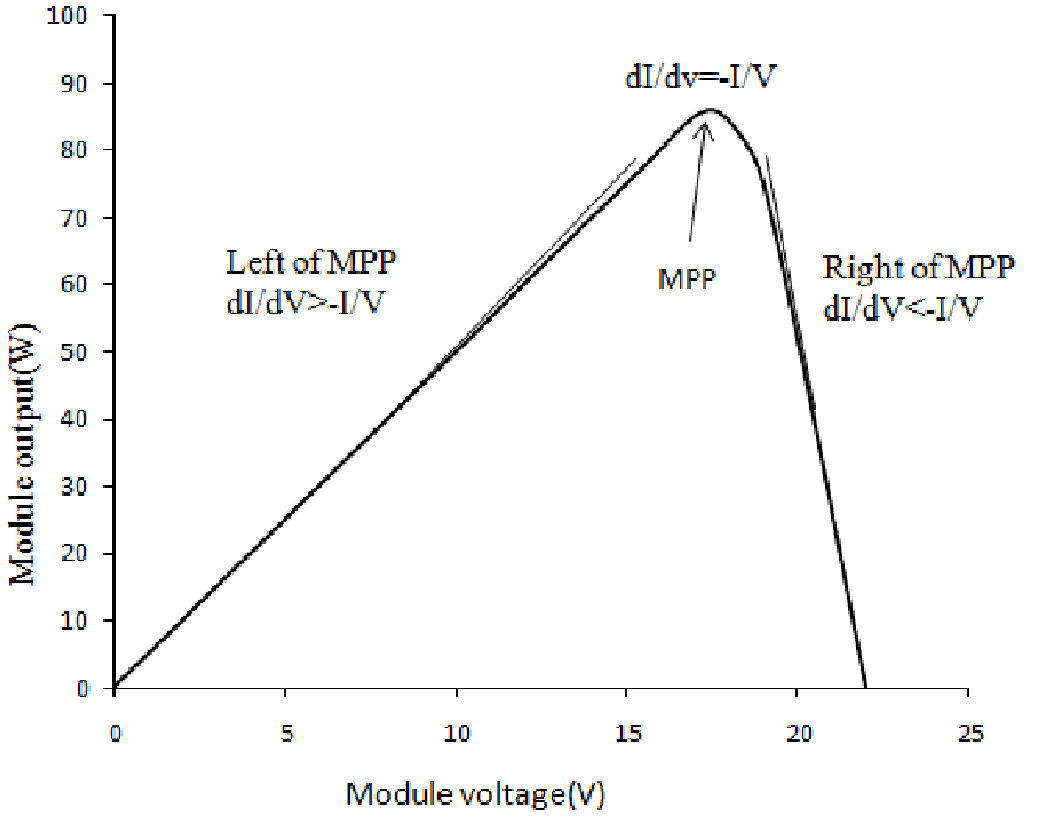
\includegraphics[width=\textwidth]{Images/Background/InCond_graph.pdf}
                \caption{\ac{incond} method principle.}
                \label{fig:IncCond_graph}
            \end{minipage}
        \end{figure}

    
        \subsection{Look Up Table (LUT)}
            The \ac{lut} method is a simple and fast \ac{mppt} algorithm that relies on pre-calculated/measured data to determine the optimal operating point of a solar panel~\cite{MPPT_Comparison_techniques}.
            
            The \acs{lut} table contains several entries organized by voltage and current. Each of these entries contains the optimal duty cycle of the DC-DC converter, which is pre-calculated or measured for a specific voltage and current. This approach allows the algorithm to reach the \acs{mpp} in one clock cycle by measuring the solar panel voltage and current, finding the closest entry in the \ac{lut} table, and applying the corresponding duty cycle to the converter. The entries of the table can be calculated through a mathematical model of the solar panel with different conditions (temperature and irradiance) or measured in a laboratory.

            Table~\ref{tab:LUT_matrix} visually represents a 2D \acs{lut} based only on current and voltage. Each entry represents the duty cycle used in each case.

            The main advantage of this method is its speed since it can reach the \ac{mpp} in one clock cycle. This makes it suitable for applications that require fast tracking or use weak \acp{mcu}. However, it is not very accurate~\cite{Look-Up-Table_VS_PeO}.

            \begin{table}[ht]
                \centering
                \caption{\acs{lut} matrix representation with $m \times n$ elements.}
                \label{tab:LUT_matrix}
                \renewcommand{\arraystretch}{1.3}
                \begin{tabular}{c|ccccccc}
                    & $V_1$ & $\cdots$ & $V_k$ & $\cdots$ & $V_m$ \\
                    \hline
                    $I_1$ & $D_{11}$ & $\cdots$ & $D_{1k}$ & $\cdots$ & $D_{1m}$ \\
                    $\vdots$ & $\vdots$ &  & $\vdots$ &  & $\vdots$ \\
                    $I_j$ & $D_{j1}$ & $\cdots$ & $D_{jk}$ & $\cdots$ & $D_{jm}$ \\
                    $\vdots$ & $\vdots$ &  & $\vdots$ &  & $\vdots$ \\
                    $I_n$ & $D_{n1}$ & $\cdots$ & $D_{nk}$ & $\cdots$ & $D_{nm}$
                \end{tabular}
            \end{table}

            To improve the accuracy, the \acs{lut} table needs to be large, which increases the required memory resources. Also, by adding the temperature and/or irradiance to the table would increase the accuracy, making it almost 100\% accurate, but this would increase the size of the table exponentially. In extreme cases, the memory requirements became expensive and slow. There is a trade-off between size, speed, and accuracy that needs to be considered when using this method. Also, the \acs{lut} method does not adapt to the aging of the solar panel or changes in its characteristics over time, unless the table is updated periodically through new measurements, which adds maintenance time.
            

\section{Types of DC-DC Converters}
    The \acs{dc}-\acs{dc} converter is a crucial component of an \acs{mppt} charger because it adjusts the solar panel operating point to match the \ac{mpp}. This choice is important to the project because it directly affects the overall system's efficiency, cost, and complexity.

    \acs{dc}-\acs{dc} converters fall into two main categories: isolated and non-isolated converters. The main difference between these two types of converters is the presence or absence of galvanic isolation between the input and output circuits~\cite{flexpower_isolated_vs_nonisolated_2025}.


    \subsection{Non-isolated versus isolated DC-DC converters}
        Galvanic isolation is usually achieved by using a transformer, which provides electrical isolation between the input and output sides of the converter. This isolation is important in applications where safety is a concern, such as in medical devices or industrial equipment, as it helps to prevent electrical shock and damage to sensitive components. In solar energy systems and E-mobility, isolated converters are often used when the solar panel is connected to the grid~\cite{Review_Isolated_Non_isolated_DC_DC_Converters_MVDC_2021}, as they help protect against voltage spikes and other electrical disturbances. Also, non-isolated converters can provide much higher/lower gain, which is useful for applications where 
        solar panels \ac{mpp} voltage differs greatly from the battery or load voltage (typically medium/high voltages, which is not the case). 

        In contrast, non-isolated converters do not provide galvanic isolation between the input and output circuits. However, they generally offer higher efficiency, lower cost, reduced size, and lower circuit complexity (Table~\ref{tab:switching-vs-isolated-converters}). They also pose fewer thermal management challenges and are simpler to design. These advantages, along with the fact that galvanic isolation is not required for this application, led to excluding isolated \acs{dc}-\acs{dc} converters from this project.

        \begin{table}[htbp]
            \centering
            \caption{Comparison between Non-isolated and isolated converters.}
            \label{tab:switching-vs-isolated-converters}
            \scriptsize
            \setlength{\tabcolsep}{5pt}
            \renewcommand{\arraystretch}{1.1}
            \begin{adjustbox}{max width=0.95\textwidth}
                \begin{tabularx}{\textwidth}{>{\raggedright\arraybackslash}p{4cm}
                                            >{\centering\arraybackslash}X
                                            >{\centering\arraybackslash}X}
                \toprule
                Type & Non-isolated Converters & Galvanic Isolated Converters \\
                \midrule

                Circuit Complexity & \G Low & \R High \\
                Efficiency & \G High & \Y Medium \\
                Size & \G Compact & \R Large \\
                Electromagnetic Interference (EMI) & \Y Medium/High &  \R High\\
                Switching Frequency & \Y Medium & \Y Medium \\
                Thermal Management & \G Easier & \Y Moderate \\
                Control Complexity & \Y Moderate & \Y Moderate \\
                Gain & \Y Near 1 & \G Very High/low \\
                Cost & \G Low & \R High \\
                \bottomrule
                \end{tabularx}
            \end{adjustbox}
            \begin{center}
                Legend: \fcolorbox{black}{light_red}{undesired} \fcolorbox{black}{light_yellow}{medium} \fcolorbox{black}{light_green}{good}
            \end{center}
        \end{table}

        
        

        
            


    \subsection{Non-isolated DC-DC converters}
        Modern non-isolated conversion circuits generally use one of three basic topologies: buck, boost, or buck-boost converters. They are "basic" in the sense that only one switching element is needed. Each topology provides a specific result, such as voltage step-down, voltage step-up, or hybrid mode~\cite{Comparison_PV_Converter_Technologies_1989}. 

            The \textbf{boost converter} is a step-up \acs{dc}-\acs{dc} converter widely employed in \ac{mppt} controllers when the required output voltage is higher than the solar panel open circuit voltage. 
            It uses an inductor to store energy when the transistor is in the ON state and a diode in reverse bias (Figure~\ref{fig:DC-DC_classic_topologys}b). When the transistor is on the OFF state, the inductor releases the stored energy to the output through the diode, increasing the output voltage ~\cite{Non_Isolated_DC_DC_Converters_MPPT_Controller_2021}.

            This topology has been extensively documented in the literature and is distinguished by its inherent simplicity, cost-effectiveness, and superior efficiency characteristics~\cite{shahira2022_electrical_design_solar_boat}\cite{Look-Up-Table_VS_PeO}\cite{Intelligent_PV_Module_2006}. Depending on the design variation used and constraints, it can achieve conversion efficiencies up to 98\%~\cite{Review_Isolated_Non_isolated_DC_DC_Converter_PV_Application_2018}. 

            A limitation of this topology is that it cannot emulate an impedance lower than the load impedance, which prevents it from reaching values close to the short-circuit current of the \acs{pv} module. Consequently, it is not compatible with all solar panels or \acs{mppt} algorithms~\cite{Review_Isolated_Non_isolated_DC_DC_Converter_PV_Application_2018,A_New_Application_Buck_Boost_Converters_IV_Curve_PV_Modules_2007}.


            The \textbf{buck converter} is a step-down \acs{dc}-\acs{dc} converter widely used when the solar panel voltage is higher than the battery or load voltage. Similar to the boost converter, it uses an inductor to store energy when the transistor is in the ON state and the diode is reverse-biased. However, in this case, the input connects to the output when the transistor is in the ON state. When the transistor is in the OFF state, the inductor releases the stored energy to the output through the diode, decreasing the output voltage (Figure~\ref{fig:DC-DC_classic_topologys}a)~\cite{Review_Isolated_Non_isolated_DC_DC_Converter_PV_Application_2018}.

            This converter also has a similar downside to the boost converter. The buck converter can not emulate a smaller impedance than the load impedance, and therefore, it can not reach values near the open circuit voltage of the PV module~\cite{Review_Isolated_Non_isolated_DC_DC_Converter_PV_Application_2018}\cite{A_New_Application_Buck_Boost_Converters_IV_Curve_PV_Modules_2007}.

            \textbf{Buck-Boost converters} are step-up and step-down \acs{dc}-\acs{dc} converters that can operate in both modes. This makes them more versatile than the previous two topologies, but also more complex and less efficient~\cite{Review_Isolated_Non_isolated_DC_DC_Converter_PV_Application_2018}. This converter uses an inductor to store energy when the transistor is in the ON state and the diode is reverse-biased. When the transistor is in the OFF state, the inductor releases the stored energy to the output through the diode, increasing or decreasing the output voltage (Figure~\ref{fig:DC-DC_classic_topologys}c)~\cite{Comparison_PV_Converter_Technologies_1989}.

            \begin{figure} [!ht]
                \centering
                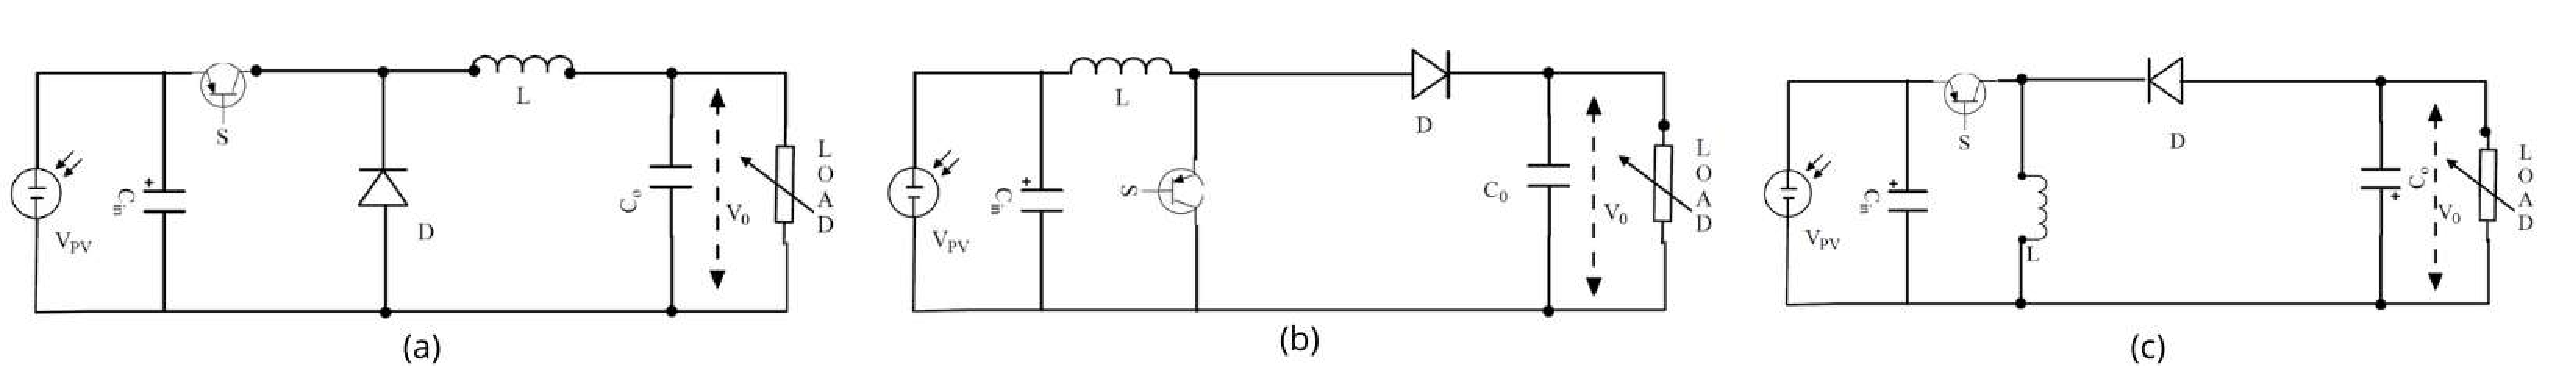
\includegraphics[width= \textwidth]{Images/Background/DC-DC_classic_topologys.pdf}
                \qquad
                \caption{Buck (a), Boost (b) and Buck-Boost (c) DC-DC converters.}
                \label{fig:DC-DC_classic_topologys}
            \end{figure}
 
            The conventional buck-boost converter produces an output voltage inverted relative to the input, which creates challenges for sensor measurements, driving circuits, and isolation, consequently, this option was excluded for the current project \cite{Non_Isolated_DC_DC_Converters_MPPT_Controller_2021}.


            An enhanced variant of the buck-boost converter is the CUK converter, illustrated in Figure~\ref{fig:DC-DC_buck_bost}a. The main characteristic of the CUK converter is that the currents through inductors $L_1$ and $L_2$ are equal, allowing the use of a common magnetic core, which helps reduce current ripple. However, a major drawback of this topology is that the entire load current must pass through the coupling capacitor $C$. In addition, the converter produces an inverted output voltage~\cite{Non_Isolated_DC_DC_Converters_MPPT_Controller_2021}.

            The issue of output voltage polarity inversion can be addressed by using a single-ended primary inductor converter (SEPIC), as shown in Figure~\ref{fig:DC-DC_buck_bost}b. Nevertheless, its main drawbacks are the high output current and voltage ripple which increases losses and electromagnetic interference (EMI)~\cite{Comparative_Analysis_Non_Isolated_DC_DC_Converters_Solar_PV_2021}. The ZETA converter, shown in Figure~\ref{fig:DC-DC_buck_bost}c, mitigates these limitations by improving output current characteristics while maintaining the same output voltage polarity as the SEPIC converter~\cite{PeO_and_Newton_Raphson_Comparison}\cite{Non_Isolated_DC_DC_Converters_MPPT_Controller_2021}.

            \begin{figure} [!ht]
                \centering
                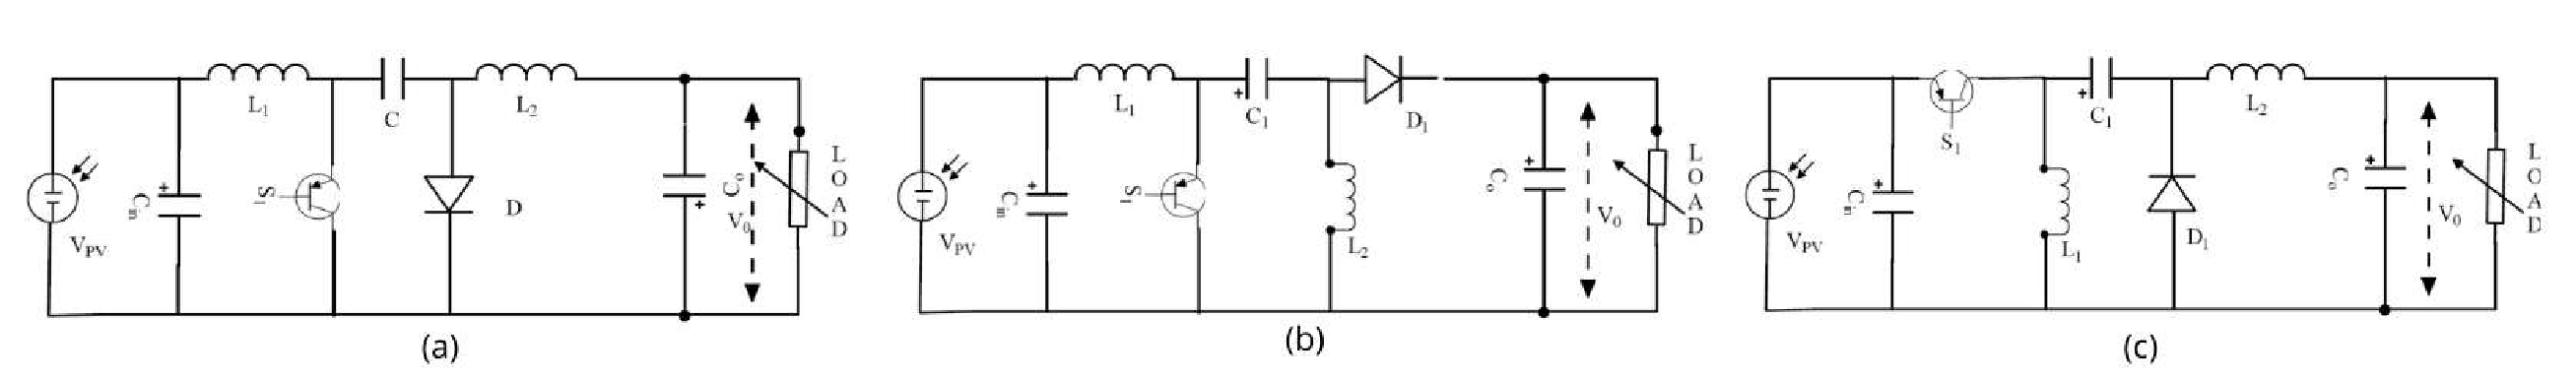
\includegraphics[width= \textwidth]{Images/Background/DC-DC_buck_bost.pdf}
                \qquad
                \caption{CUK (a), SEPIC (b) and ZETA (c) DC-DC converters.}
                \label{fig:DC-DC_buck_bost}
            \end{figure}

            % Landsman converter is another alternative that provides low input current ripple and non-inverted output voltage while keeping a good efficiency. However, it has high voltage and current output ripple, which is not ideal for battery charging applications~\cite{Comparative_Analysis_Non_Isolated_DC_DC_Converters_Solar_PV_2021}.



    \subsection{Comparison between Non-isolated DC-DC converters}
        All the non-isolated \acs{dc}-\acs{dc} topologies explained before have their own advantages and disadvantages. The choice of topology depends on the specific application, desired performance, and available resources. To help with this choice, Table~\ref{tab:dc-dc-comparison} shows a comparison between the most relevant characteristics of each topology~\cite{Comparative_Analysis_Non_Isolated_DC_DC_Converters_Solar_PV_2021}. The most significant advantages of each topology are highlighted according to the project's aim.

        \begin{table}[htbp]
        \centering
        \caption{Comparison of non-isolated DC-DC topologies.}
        \label{tab:dc-dc-comparison}
        \scriptsize
        \setlength{\tabcolsep}{4pt}
        \renewcommand{\arraystretch}{1.05}
        \begin{adjustbox}{max width=0.95\textwidth}
            \begin{tabularx}{\textwidth}{>{\raggedright\arraybackslash}p{2.7cm}
                                        >{\centering\arraybackslash}X
                                        >{\centering\arraybackslash}X
                                        >{\centering\arraybackslash}X
                                        >{\centering\arraybackslash}X
                                        >{\centering\arraybackslash}X
                                        >{\centering\arraybackslash}X}
            \toprule
            \textbf{Topology} & \textbf{Boost} & \textbf{Buck} & \textbf{Buck-Boost} & \textbf{ZETA} & \textbf{CUK} & \textbf{SEPIC} \\
            \midrule
            \multicolumn{7}{l}{\textit{\textbf{Electrical performance}}} \\
            Efficiency & \DG High & \DG High & \DG High & \DG Medium/High &  Medium & Medium \\
            EMI & \G Low & \G Low & High & Medium & Medium & Medium \\
            Input current ripple & \G Low  & High & High & \G Low & \G Very low & Medium \\
            Output current ripple & High & \G Low & High & \G Very low & \G Low & Medium \\
            Output voltage ripple & Medium & \DG Low & Medium & \DG Low & Medium & High \\
            \midrule
            \multicolumn{7}{l}{\textit{\textbf{Structural characteristics}}} \\
            Circuit complexity & \G Low & \G Low & \G Low & Medium & Medium & Medium \\
            Size & \G Low & \G Low & \G Low & Medium & Medium & Medium \\
            Storage elements & \G 1 L & \G 1 L & \G 1 L & 2 L, 1 C & 2 L, 1 C & 2 L, 1 C \\
            Switch stress & \G No & Yes & \G No & Yes & Yes & Yes \\
            \midrule
            \multicolumn{7}{l}{\textit{\textbf{Functional aspects}}} \\
            Type & \G Step-Up & Step-Down & \DG Step-Down/Up & \DG Step-Down/Up & \DG Step-Down/Up & \DG Step-Down/Up \\
            Versatility & Low & Low & Medium & \G High & Medium & \G High \\
            Inverted output & \G No & \G No & Yes & \G No & Yes & \G No \\
            Reliability & \G High & \G High & \G High & Medium & Medium & Medium \\
            \midrule
            \multicolumn{7}{l}{\textit{\textbf{Economic}}} \\
            Cost & \DG Low & \DG Low & \DG Low & Medium & Medium & Medium \\
            \bottomrule
            \end{tabularx}
        \end{adjustbox}
            \begin{center}
                Legend: \fcolorbox{black}{light_green}{good} \fcolorbox{black}{dark_green}{important}
            \end{center}
        \end{table}

        For \acs{mppt} controllers, the choice is mainly governed by the ability to operate at the \ac{mpp}, which depends on the converter type (Step Up, Down, or Down/Up). Efficiency, cost (related to the number of storage elements), and output voltage ripple are also relevant to this choice.

        The buck converter can be excluded from this comparison since, in this project, the solar panel voltage is lower than the battery voltage, therefore, a step-down converter is not suitable.
        However, when choosing between the boost and the step-up/down converters, there is a trade-off. 
        The boost converter is simpler, cheaper, and more efficient. On the other hand, step-up/down converters are more versatile because they can operate over a wide range of input voltages, which is useful since solar panel size and battery voltage can change.

        Since the solar panel voltage is always lower than the battery voltage in this project, the boost converter is the most suitable topology because of its simplicity, cost-effectiveness, and high efficiency. However, if versatility were to become a priority, the ZETA converter would be the preferred choice among the step-up/down topologies, owing to its non-inverted output voltage and low output current ripple, which are advantageous for battery charging applications.

    
\section{Battery charging techniques}

    As the demand for electronic devices and E-vehicles increases, the need for efficient, compact, and lightweight batteries has emerged. Among many existing technologies, lithium-ion batteries have one of the best energy-to-weight/volume ratios and, at this moment, it is the technology used in \ac{tsb} batteries. But like every other battery technology, they must be charged properly to ensure safety and longevity~\cite{Charging_Algorithms_Lithium_Ion_Batteries_Overview_2012}.

    To charge these batteries properly, the \ac{mppt} algorithm can operate alone if an additional converter is used in series. But in most of \ac{mppt} chargers, the \ac{mppt} and the battery charging unit are integrated in the same converter. This way, the \ac{mppt} algorithm can adjust the solar panel operating point to extract maximum power, while the battery charging technique ensures the battery charges properly. A proper combination of both algorithms/techniques is essential to ensure both maximum energy extraction and safe battery charge.

    Several charging techniques are available for lithium-ion batteries. For the application considered in this work, the most relevant approach is the constant-current constant-voltage (\acs{cc}-\acs{cv}) charging method~\cite{Charging_Algorithms_Nickel_Lithium_Battery_2011}.It is also widely used in commercial chargers because of its simplicity and effectiveness~\cite{Review_Different_Charging_Techniques_Lithium_Polymer_Battery_2015}. 
    This method consists of two main phases (Figure~\ref{fig:CC-CV profile}). In the first phase, the battery is charged at a constant current until it reaches its maximum voltage. In the second phase, the voltage is held constant at this limit while the current gradually decreases as the battery approaches full charge. Once the current drops below a certain threshold, the charging process is terminated to prevent overcharging~\cite{Review_Different_Charging_Techniques_Lithium_Polymer_Battery_2015}.

    When employing the \acs{cc}-\acs{cv} charging technique with a \ac{mppt} controller, the initial \ac{cc} phase is regulated by the \ac{mppt} algorithm, which extracts the maximum available power from the solar panel, limited by the maximum charging current. Once the maximum charge current is reached, it operates at \ac{cc}. Once the \ac{cv} phase is reached, the \ac{mppt} function is disabled, and the power converter increases the solar panel voltage to progressively reduce the charging current while keeping the output voltage constant.


    \begin{figure} [!ht]
        \centering
        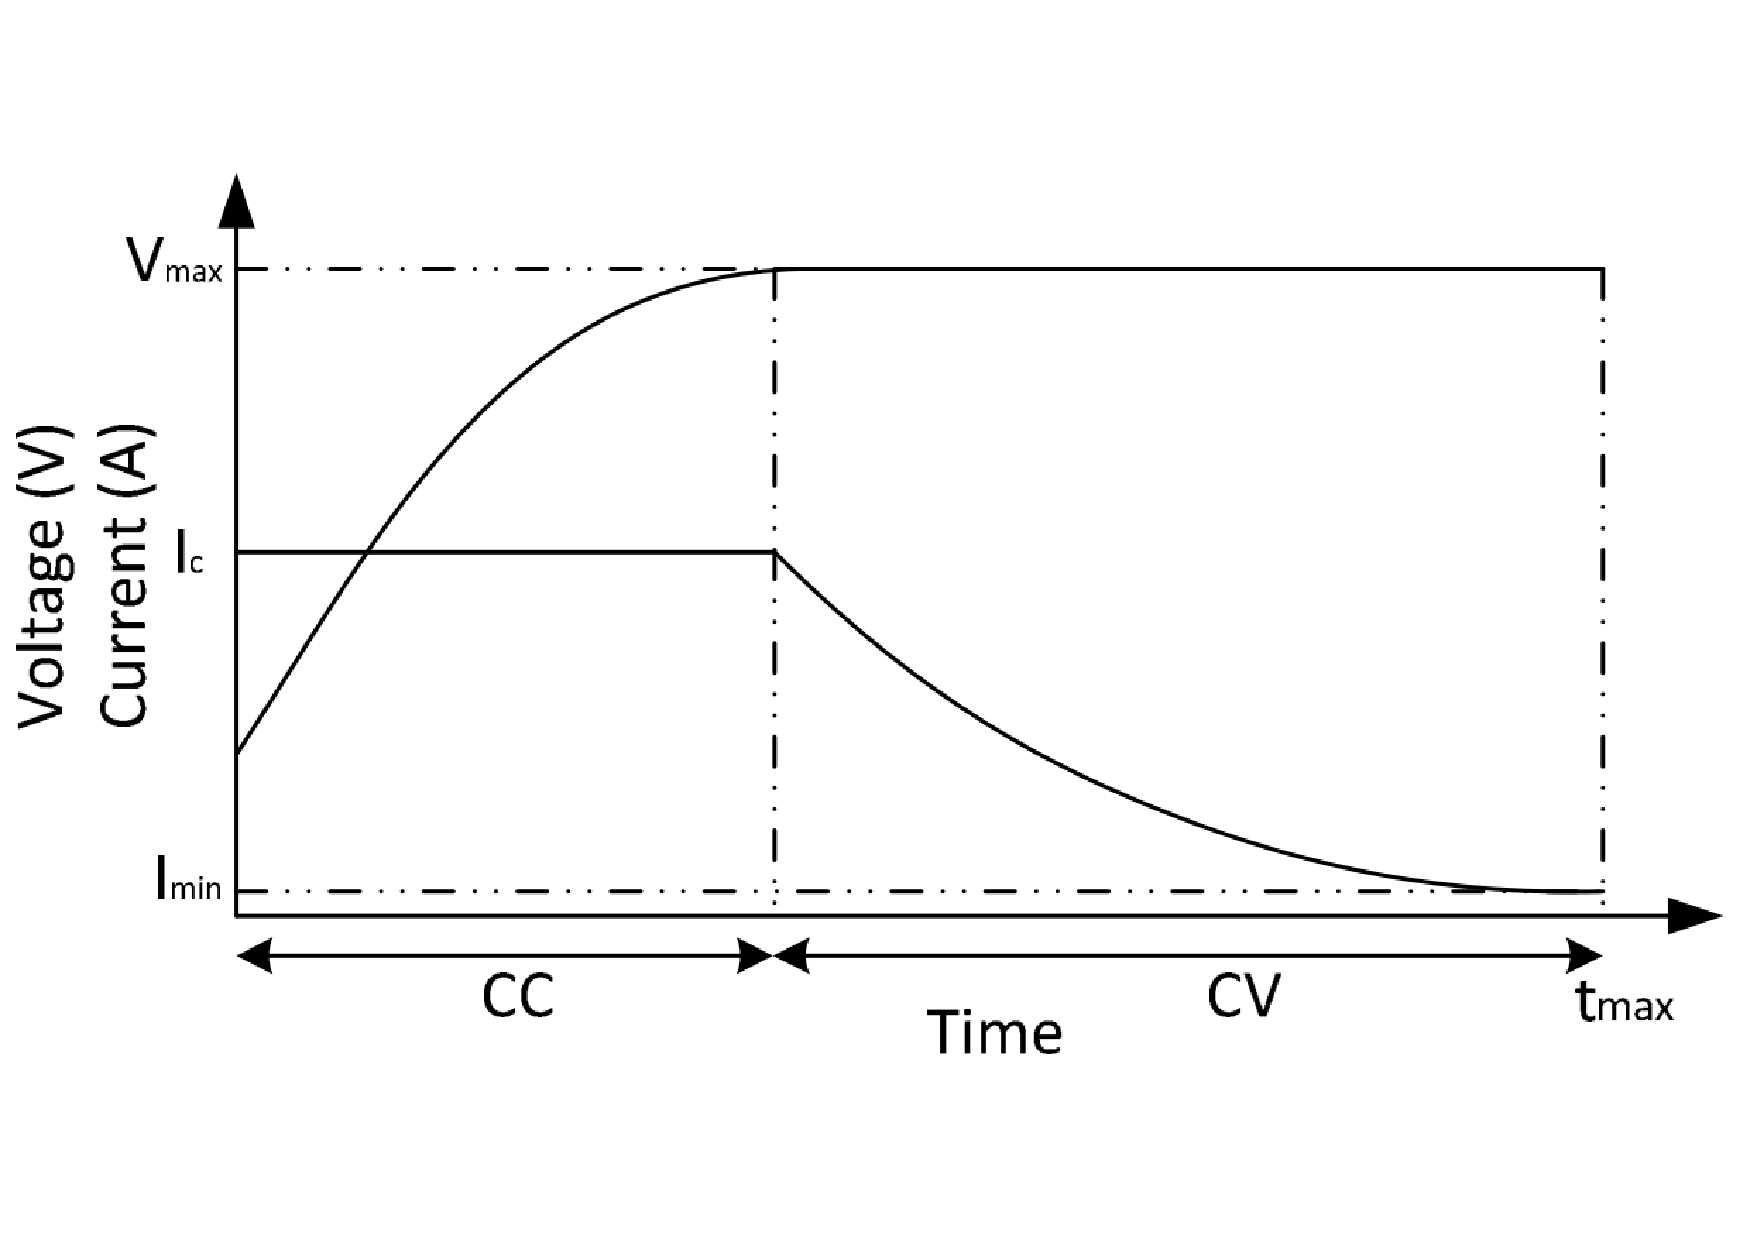
\includegraphics[width=0.45 \textwidth]{Images/Background/CC-CV graph.pdf}
        \qquad
        \caption{Charging profile of CC/CV~\cite{Charging_Algorithms_Lithium_Ion_Batteries_Overview_2012}.}
        \label{fig:CC-CV profile}
    \end{figure}

    The literature has proposed more advanced high-performance battery charging techniques to reduce charging time without increasing charging current, thereby preserving battery lifetime. However, these techniques generally introduce higher switching losses and increased system complexity. In the present application, the current generated by the photovoltaic panels is less than half of the maximum allowable battery charging current, consequently, the charging current is inherently limited by the solar panels rather than by the charging strategy. Furthermore, battery lifetime is not a critical concern in this project, as the battery is expected to undergo a limited number of charge cycles, not exceeding 20 cycles per year.

    Therefore, the \acs{cc}-\acs{cv} charging method is considered the most suitable technique for this project, owing to its simplicity, effectiveness, and widespread adoption in commercial battery chargers. 

    Other charging techniques fall outside the scope of this work, however, some methods are briefly discussed in the references provided~\cite{Charging_Algorithms_Nickel_Lithium_Battery_2011}\cite{Charging_Algorithms_Lithium_Ion_Batteries_Overview_2012}\cite{Review_Different_Charging_Techniques_Lithium_Polymer_Battery_2015}.

    


        % \textcolor{red}{If there is time, chose a specific STM32 and justify the choice based on some parameters.}



\section{Commercial Options}
    To assess the feasibility of adopting a \ac{ots} solution, this section reviews existing commercial options for solar battery charging with \ac{mppt} capability. Both specialized \acp{ic} and complete commercial \ac{mppt} chargers are considered, and their electrical, functional, and economic characteristics are evaluated against the requirements of this project. The objective is to identify whether a commercially available solution can satisfy the constraints of the application or, alternatively, to justify the need for a custom designed converter and control system.

\subsection{Specialized ICs}
\label{sec:ICs}
    Several commercially available \acf{ic} are specifically designed for solar battery charging and \ac{mppt} applications. These devices are relevant to this project since, if suitable, they could significantly reduce design complexity by integrating functions such as \acs{dc}-\acs{dc} conversion, protection mechanisms, and an \acs{mppt} algorithm.

    Table~\ref{tab:commercial-ics-comparison} summarizes four commonly used commercial \acp{ic}. Characteristics marked in red indicate incompatibilities with the project requirements, leading to the exclusion of the corresponding devices.

    The BQ24650RVAT is a stand-alone synchronous buck battery charge controller that implements a high-efficiency battery charger and provides safety features. By adding a \ac{mcu} to run a \acs{mppt} algorithm and current and voltage sensors, this \acs{ic} can track the \ac{mpp} of a solar panel, making it appropriate for applications with 12/24~V batteries and high-power panels, such as electric vehicles. However, it does not support the required 48~V battery voltage and is therefore unsuitable for this work.

    The MAX20801TPBA+ and SPV1040TTR target low-power IoT applications with small batteries and solar panels. Both devices cannot meet the 48~V output requirement, and limited publicly available information on tracking speed further restricts performance evaluation.

    The LT8491IUKJ\#PBF offers a wide input and output voltage range, buck-boost operation, high efficiency, communication capabilities, and \acs{cc}-\acs{cv} charging. Despite these advantages, its reported \acs{mppt} tracking speed of up to 2~s is insufficient for the dynamic conditions of this application. Additionally, its I\textsuperscript{2}C interface would require an additional microcontroller to provide \acs{can} communication, increasing system cost.

    \begin{table}[htbp]
        \centering
        \caption{Comparison of commercial specialized \acp{ic}.}
        \label{tab:commercial-ics-comparison}
        \scriptsize
        \setlength{\tabcolsep}{4pt}
        \renewcommand{\arraystretch}{1.05}
        \begin{adjustbox}{max width=0.95\textwidth}
        \begin{tabularx}{\textwidth}{>{\raggedright\arraybackslash}p{2.7cm}
                                    >{\centering\arraybackslash}X
                                    >{\centering\arraybackslash}X
                                    >{\centering\arraybackslash}X
                                    >{\centering\arraybackslash}X}
        \toprule
        \textbf{Model} & \textbf{BQ24650RVAT} & \textbf{MAX20801TPBA+} & \textbf{SPV1040TTR} & \textbf{LT8491IUKJ\#PBF} \\
        \midrule

        \multicolumn{5}{l}{\textit{\textbf{Electrical specifications}}} \\
        Input voltage & \R 5 to 28~V & \R 1.5 to 18~V & \R 0.3 to 5.5~V & 6 to 80~V \\
        Output voltage & \R 12 to 24~V & \R 12.4~V & \R -0.3 to 5.5~V & 1.3 to 80~V \\
        Max output current & Externally limited & 12~A & \R 1.8~A & 10~A \\
        Switching frequency & 600~kHz & Unknown & 100~kHz & 100 to 400~kHz \\
        Electrical efficiency & 95\% & 99.1\% (max) & \R 80 to 95\% & 95 to 99\% \\

        \midrule
        \multicolumn{5}{l}{\textit{\textbf{MPPT and control}}} \\
        Algorithm & User input & Unknown & Unknown & P\&O \\
        Tracking accuracy & User dependent & 99.9\% (max) & \R Unknown & \R Unknown \\
        Tracking speed & User dependent & \R Unknown & \R Unknown & \R 1 to 2~s \\

        \midrule
        \multicolumn{5}{l}{\textit{\textbf{Functional aspects}}} \\
        Topology & Synchronous Buck & Synchronous Buck & Synchronous Boost & Buck-Boost \\
        Communication & \R No & \R No & \R No & \R I\textsuperscript{2}C \\
        Configurability & No & No & No & Yes \\
        Charge profile & CC-CV & \R Unknown & \R Unknown & CC-CV \\
        \midrule
        \multicolumn{5}{l}{\textit{\textbf{Extra hardware needed}}} \\
        Transistors &  Yes & No & No &  Yes \\
        Sensors & Yes & No & No & No \\
        Storage elements & Yes & Yes & Yes & Yes \\

        \midrule
        \multicolumn{5}{l}{\textit{\textbf{Economic}}} \\
        Price & 5.25~€ & 4.50~€ & 3.02~€ & \R 15-20~€ \\

        \bottomrule
        \end{tabularx}
        \end{adjustbox}
        \begin{center}
            Legend: \fcolorbox{black}{light_red}{unsuitable}
        \end{center}
    \end{table}


\subsection{Commercial MPPT chargers}
Several commercial \ac{mppt} chargers can address the problem under analysis without requiring additional hardware. However, each solution presents limitations when evaluated against the project requirements. Table~\ref{tab:commercial-mppt-comparison} summarizes selected commercial \acs{mppt} chargers, with red-marked characteristics indicating incompatibilities.

The GVB-8-Li-CV(50.4) is a high-performance and fast \ac{mppt} charger, particularly suited for dynamic environments such as marine applications. It has been successfully used by \acs{tsb} in previous projects, demonstrating high efficiency and reliability. Nevertheless, its lack of configurability, fixed output voltage, no communication and high cost restrict its suitability for this application. Despite these drawbacks, it serves as a valuable reference design.

The Smart Solar MPPT 100/20, developed by Victron Energy, offers high efficiency, fast tracking, and integrated communication interfaces. However, it uses a buck topology that requires higher input voltages, making it incompatible with the small and distributed solar panel arrays used in the \acs{tsb} application.

Other commercial solutions, such as the Rover Lite and MS4840N, provide acceptable performance but rely on communication protocols incompatible with the project requirements and offer limited technical documentation.

The Reboost V0.2.1 is an open source \ac{mppt} charger originally developed for automotive applications. While it provides flexibility and near adequate specifications, its reliance on expensive and discontinued components, along with the use of a boost topology, limits scalability and adaptability to potential future battery voltage changes.

Overall, none of the evaluated commercial \ac{mppt} chargers fully satisfy the technical, economic, and configurability requirements of this project, motivating the development of a custom solution.

    \begin{table}[htbp]
        \centering
        \caption{Comparison of commercial MPPT controllers.}
        \label{tab:commercial-mppt-comparison}
        \scriptsize
        \setlength{\tabcolsep}{3pt}
        \renewcommand{\arraystretch}{1.05}
        \begin{adjustbox}{max width=0.95\textwidth}
        \begin{tabularx}{\textwidth}{>{\raggedright\arraybackslash}p{2.5cm}
                                    >{\centering\arraybackslash}X
                                    >{\centering\arraybackslash}X
                                    >{\centering\arraybackslash}X
                                    >{\centering\arraybackslash}X
                                    >{\centering\arraybackslash}X}
        \toprule
        \textbf{Model} & \textbf{GVB-8-Li-CV (50.4V)} & \textbf{Smart Solar MPPT 100/20} &
        \textbf{Reboost V0.2.1} & \textbf{Rover Lite} & \textbf{MS4840N} \\
        \midrule

        \multicolumn{6}{l}{\textit{\textbf{General information}}} \\
        Brand & Gensun & Victron Energy & TPEE & Renogy & BougeRV \\
        Type & Boost & \R Buck & Synchronous Boost & Boost & Boost \\

        \midrule
        \multicolumn{6}{l}{\textit{\textbf{Control and communication}}} \\
        Communication & \R No &
        \R VE.can and Bluetooth &
        Yes &
        \R Bluetooth and RS485 &
        \R Bluetooth \\
        Configurable & \R No & Yes & Yes & Yes & Yes \\
        GUI & No & Yes & Yes & Yes & Yes \\

        \midrule
        \multicolumn{6}{l}{\textit{\textbf{MPPT and charging}}} \\
        Prog. battery voltage &
        \R No &
        Yes &
        Yes &
        \R non-lithium batteries &
        Yes \\
        Tracking speed &
        15~Hz / 66.6(6)~ms &
        \R Fast (unknown) &
        Programmable &
        \R Unknown &
        \R Unknown \\
        Tracking efficiency &
        99\%+ typical &
        \R Unknown &
        Programmable &
        99\% &
        \R Unknown \\
        Electrical efficiency &
        96-99\% typical &
        98\% peak &
        \R Unknown &
        97\% &
        \R Unknown \\
        Charger profile &
        CC-CV &
        \R Unknown &
        Programmable &
        \R Unknown &
        CC-CV \\

        \midrule
        \multicolumn{6}{l}{\textit{\textbf{Hardware implementation}}} \\
        MCU & ATtiny461A-U & Unknown & STM32G474 & Unknown & Unknown \\
        MCU Details &
        8-bit, RISC, 64~MHz &
        -- &
        32-bit, Arm, 170~MHz  &
        -- &
        -- \\
        Transistor &
        FZT951  &
        Unknown &
        GS61008T  &
        Unknown &
        Unknown \\
        Transistor type & PNP BJT & Unknown & GaN FETs & Unknown & Unknown \\

        \midrule
        \multicolumn{6}{l}{\textit{\textbf{Economic}}} \\
        Price &
        \R 240~€ &
        \R 100-200~€ &
        \R Components: 250-280~€ \newline PCB: 20-100~€ \newline Total: 270-380~€ &
        \R 300-350~€ &
        \R 120-160~€ \\

        \bottomrule
        \end{tabularx}
        \end{adjustbox}
            \begin{center}
                Legend: \fcolorbox{black}{light_red}{unsuitable}
            \end{center}
        \end{table}

    